%%%%%%%%%%%%%%
%% Run LaTeX on this file several times to get Table of Contents,
%% cross-references, and citations.


% 6x9

\documentclass{wileySix}

\documentclass{wileysix}


\usepackage{graphicx}
\usepackage{listings}

\usepackage{color}
 
\definecolor{codegreen}{rgb}{0,0.6,0}
\definecolor{codegray}{rgb}{0.5,0.5,0.5}
\definecolor{codepurple}{rgb}{0.58,0,0.82}
\definecolor{backcolour}{rgb}{0.95,0.95,0.92}
 
\lstdefinestyle{mystyle}{
    backgroundcolor=\color{backcolour},   
    commentstyle=\color{codegreen},
    keywordstyle=\color{magenta},
    numberstyle=\tiny\color{codegray},
    stringstyle=\color{codepurple},
    basicstyle=\footnotesize,
    breakatwhitespace=false,         
    breaklines=true,                 
    captionpos=b,                    
    keepspaces=true,                 
    numbers=left,                    
    numbersep=5pt,                  
    showspaces=false,                
    showstringspaces=false,
    showtabs=false,                  
    tabsize=2,
    language=sh
}
 
\lstset{style=mystyle}

%%%%%%%
%% for times math: However, this package disables bold math (!)
%% \mathbf{x} will still work, but you will not have bold math
%% in section heads or chapter titles. If you don't use math
%% in those environments, mathptmx might be a good choice.

% \usepackage{mathptmx}

% For PostScript text
\usepackage{w-bookps}

%%%%%%%%%%%%%%%%%%%%%%%%%%%%%%%%%%%%%%%%%%%%%%%%%%%%%%%%%%%%%%%%
%% Other packages you might want to use:

% for chapter bibliography made with BibTeX
% \usepackage{chapterbib}

% for multiple indices
% \usepackage{multind}

% for answers to problems
% \usepackage{answers}

%%%%%%%%%%%%%%%%%%%%%%%%%%%%%%
%% Change options here if you want:
%%
%% How many levels of section head would you like numbered?
%% 0= no section numbers, 1= section, 2= subsection, 3= subsubsection
%%==>>
\setcounter{secnumdepth}{3}

%% How many levels of section head would you like to appear in the
%% Table of Contents?
%% 0= chapter titles, 1= section titles, 2= subsection titles, 
%% 3= subsubsection titles.
%%==>>
\setcounter{tocdepth}{2}

%% Cropmarks? good for final page makeup
%% \docropmarks

%%%%%%%%%%%%%%%%%%%%%%%%%%%%%%
%
% DRAFT
%
% Uncomment to get double spacing between lines, current date and time
% printed at bottom of page.
% \draft
% (If you want to keep tables from becoming double spaced also uncomment
% this):
% \renewcommand{\arraystretch}{0.6}
%%%%%%%%%%%%%%%%%%%%%%%%%%%%%%

%%%%%%% Demo of section head containing sample macro:
%% To get a macro to expand correctly in a section head, with upper and
%% lower case math, put the definition and set the box 
%% before \begin{document}, so that when it appears in the 
%% table of contents it will also work:



%% use a box to expand the macro before we put it into the section head:

\newbox\sectsavebox
\setbox\sectsavebox=\hbox{\boldmath\VT{xyz}}

%%%%%%%%%%%%%%%%% End Demo


\begin{document}



\booktitle{PHP7: Buku Belajar Untuk Pemula Dan Awam Pemrograman }
\subtitle{Dalam 24 Jam}

\authors{Rolly M. Awangga\\
\affil{Informatics Research Center}




\offprintinfo{PHP7: Buku Belajar Untuk Pemula Dan Awam Pemrograman, First Edition}{Rolly M. Awangga}


%% Can use \\ if title, and edition are too wide, ie,
%% \offprintinfo{Survey Methodology,\\ Second Edition}{Robert M. Groves}

%%%%%%%%%%%%%%%%%%%%%%%%%%%%%%
%% 
\halftitlepage

\titlepage


\begin{copyrightpage}{2019}
%Survey Methodology / Robert M. Groves . . . [et al.].
%\       p. cm.---(Wiley series in survey methodology)
%\    ``Wiley-Interscience."
%\    Includes bibliographical references and index.
%\    ISBN 0-471-48348-6 (pbk.)
%\    1. Surveys---Methodology.  2. Social 
%\  sciences---Research---Statistical methods.  I. Groves, Robert M.  II. %
%Series.\\
%
%HA31.2.S873 2007
%001.4'33---dc22                                             2004044064
\end{copyrightpage}

\dedication{`Jika Kamu tidak dapat menahan lelahnya belajar, 
Maka kamu harus sanggup menahan perihnya Kebodohan.'
~Imam Syafi'i~}

\begin{contributors}
\name{Rolly Maulana Awangga,} Informatics Research Center., Politeknik Pos Indonesia, Bandung,
Indonesia



\end{contributors}

\contentsinbrief
\tableofcontents
\listoffigures
\listoftables
\lstlistoflistings


\begin{foreword}
Sepatah kata dari Kaprodi, Kabag Kemahasiswaan dan Mahasiswa
\end{foreword}

\begin{preface}
Buku ini diciptakan bagi yang awam dengan git sekalipun.

\prefaceauthor{R. M. Awangga}
\where{Bandung, Jawa Barat\\
Februari, 2019}
\end{preface}


\begin{acknowledgments}
Terima kasih atas semua masukan dari para mahasiswa agar bisa membuat buku ini 
lebih baik dan lebih mudah dimengerti.

Terima kasih ini juga ditujukan khusus untuk team IRC yang 
telah fokus untuk belajar dan memahami bagaimana buku ini mendampingi proses 
Intership.
\authorinitials{R. M. A.}
\end{acknowledgments}

\begin{acronyms}
\acro{ACGIH}{American Conference of Governmental Industrial Hygienists}
\acro{AEC}{Atomic Energy Commission}
\acro{OSHA}{Occupational Health and Safety Commission}
\acro{SAMA}{Scientific Apparatus Makers Association}
\end{acronyms}

\begin{glossary}
\term{git}Merupakan manajemen sumber kode yang dibuat oleh linus torvald.

\term{bash}Merupakan bahasa sistem operasi berbasiskan *NIX.

\term{linux}Sistem operasi berbasis sumber kode terbuka yang dibuat oleh Linus Torvald
\end{glossary}

\begin{symbols}
\term{A}Amplitude

\term{\hbox{\&}}Propositional logic symbol 

\term{a}Filter Coefficient

\bigskip

\term{\mathcal{B}}Number of Beats
\end{symbols}

\begin{introduction}

%% optional, but if you want to list author:

\introauthor{Rolly Maulana Awangga, S.T., M.T.}
{Informatics Research Center\\
Bandung, Jawa Barat, Indonesia}

Pada era disruptif  \index{disruptif}\index{disruptif!modern} 
saat ini. git merupakan sebuah kebutuhan dalam sebuah organisasi pengembangan perangkat lunak.
Buku ini diharapkan bisa menjadi penghantar para programmer, analis, IT Operation dan Project Manajer.
Dalam melakukan implementasi git pada diri dan organisasinya.

Rumusnya cuman sebagai contoh aja biar keren\cite{awangga2018sampeu}.

\begin{equation}
ABC {\cal DEF} \alpha\beta\Gamma\Delta\sum^{abc}_{def}
\end{equation}

\end{introduction}

%%%%%%%%%%%%%%%%%%Isi Buku_

\chapter{Judul Bagian Pertama}
<<<<<<< HEAD
\section{Pendahuluan}
	Situs web merupakan suatu layanan yang menyajikan informasi menggunakan konsep hyperlink, yang memudahkan pengguna dalam menelusuri atau mencari informasi dari internet untuk mendapatkan informasi, dengan cukup mengklik suatu link beupa teks atau gambar, maka dari teks atau gambar tersebut akan menampilkan informasi yang detail (rinci).
Informasi yang akan disajikan dalam halaman web menggunakan konsep multimedia, informasi dapat disajikan dengan menggunakan banyak media (teks, gambar, animasi, suara (audio), dan film). Dalam suatu halaman web, informasi akan disajikan dalam kombinasi dari media-media tersebut yang disajikan dalam suatu halaman.
	Situs web berupa kumpulan informasi yang disediakan secara perorangan, kelompok, atau organisasi. yang ditempatkan setidaknya pada sebuah server web yang dapat diakses melalui jaringan seperti Internet, ataupun jaringan wilayah lokal (LAN) melalui alamat Internet yang dikenali sebagai URL. Gabungan atas semua situs yang dapat diakses publik di Internet disebut pula sebagai World Wide Web atau lebih dikenal dengan singkatan WWW. Web merupakan hal yang sangat populer di lingkungan pengguna internet dalam mengakses dan mendapatkan informasi karena kemudahan yang diberikan kepada pengguna internet untuk melakukan penelusuran, penjelajahan dan pencarian informasi    
=======
\section{Pengenalan}
PHP adalah bahasa pemrograman script server-side yang didesain untuk pembuatan atau pengembangan web.
Dengan ini, PHP juga dapat digunakan sebagai bahasa pemrograman umum. PHP sendiri dikembangkan pada tahun 1995
oleh Rasmus Lerdorf, dan pada akhhirnya dikelola oleh The PHP Group. Situs resmi PHP beralamat http://www.php.net.
\par
PHP disebut bahasa pemrograman server side karena PHP diproses pada komputer server. 
Hal ini berbeda dibandingkan dengan bahasa pemrograman client-side seperti JavaScript yang diproses pada web browser (client).

>>>>>>> 295bf0df4a3cb6970f347bfe2e9d9ca4d639046d


\chapter{Judul Bagian Kedua}
\section{Perintah Navigasi}
Perintah navigasi direktori


\chapter{Dasar Penulisan PHP Sederhana}
\section{Aturan Dasar Penulisan Kode PHP}
Seperti bahasa pemograman yang lain, PHP juga memiliki aturan penulisan seperti case sensitifity (perbedaan antara huruf besar dan kecil), cara mengakhiri sebuah baris perintah, dan pengaruh penggunakan spasi dalam membuat kode program PHP. Berikut adalah aturan dasar penulisan kode PHP:
\subsection{Case Sensitivity (perbedaan huruf besar dan kecil) dalam PHP}
PHP tidak membedakan huruf besar dan kecil (case insensitive) untuk penamaan fungsi (function), nama class, maupun keyword bawaan PHP seperti echo, while, dan class. Ketiga baris berikut akan dianggap sama dalam PHP:
\begin{lstlisting}
<?php
Echo “Hello World”;
ECHO “Hello World”;
EchO “Hello World”;
?>
\end{lstlisting}
Akan tetapi, PHP membedakan huruf besar dan huruf kecil (case sensitive) untuk penamaan variabel, sehingga akan dianggap sebagai variabel yang berbeda. Sering kali error terjadi dikarenakan salah menuliskan nama variabel, yang seharusnya menggunakan huruf kecil, ditulis dengan huruf besar.
\begin{lstlisting}
<?php
$luqman="Luqman";
echo $Luqman; // Notice: Undefined variable: Luqman
?>
\end{lstlisting}
Untuk mengatasi perbedaan ini, disarankan menggunakan huruf kecil untuk seluruh kode PHP, termasuk variabel, fungsi maupun class. Jika membutuhkan nama variabel yang terdiri dari 2 kata, karakter spasi bisa digantikan dengan underscore.
\subsection{Karakter Spasi dan Tab dalam PHP}
Dalam PHP, karakter seperti spasi dan tab diabaikan di dalam eksekusi program PHP. Anda boleh mencoba sebuah statement menjadi beberapa baris, atau menyatukan beberapa statement dalam sebuah baris yang lumayan panjang. Seperti contoh berikut:
\begin{lstlisting}
<?php
echo "Saya belajar"; echo "Saya mengerti"; $nama="Men";
?>
\end{lstlisting}
Baris statement itu sama dengan
 \begin{lstlisting}
<?php
     echo "Saya belajar";
     echo "Saya mengerti";
     $nama = "Men";
?>
\end{lstlisting}
Walaupun contoh yang pertama lebih menghemat baris, namun lebih disarankan untuk contoh kedua, karena kita mengusahakan agar setiap statement berada dalam satu baris saja, dan menambahkan beberapa spasi di awal untuk memudahkan membaca kode program.
\par
Keuntungan penghematan baris dan beberapa byte dari sebuah file PHP tidak akan sebanding dengan mencoba memahami kode program yang dibuat dalam beberapa hari kedepan. Menambahkan sebagian komentar pada bagian kode yang lebih rumit sebagai penjelasan juga sangat disarankan.
\section{Embedded Script dan Non Embedded}
\subsection{Embedded Script}
  \item Berikut merupakan contoh dokumen HTML yang akan dihasilkan dengan menggunakan program/script PHP dalam embedded script
    Ditampilkan dibawah ini  :
    \lstinputlisting[firstline=1, lastline=12]{src/embedded_script.php}
Script diatas menunjukkan contoh script PHP sederhana yang disebut dengan script embedded yang di sisipkan diantara tag-tag HTML. Script tersebut digunakan apabila isi dari suatu dokumen HTML diinginkan dari hasil eksekusi suatu script PHP. jika dilihat dari source-nya dengan menggunakan view source pada web browser maka tampilannya akan berupa seperti berikut
    \lstinputlisting[firstline=14, lastline=22]{src/embedded_script.php}
Source dokumen HTML yang tampil berupa dokumen HTML yang tidak lagi dari script PHP yang berisi script PHP karena semua menjadi tag HTML, karena pada saat dieksekusi maka bukan scriptnya yang dikirim tetapi eksekusi dari script tersebut yang dikirim 
\subsection{Non Embedded}
   \item Script PHP dibawah ini merupakan script murni dari pembuatan program dengan menggunakan PHP, tag dokumen HTML yang dihasilkan untuk membuat dokumen merupakan bagian dari script PHP. di tampilkan dibawah ini:
  \lstinputlisting[firstline=24, lastline=35]{src/embedded_script.php}
dan dibawah ini merupakan source dokumen HTML dari tampilan kode diatas  
  \lstinputlisting[firstline=38, lastline=40]{src/embedded_script.php}
Jika diperhatikan dokumen HTML tersebut tidak beraturan ditampilkan. Hal tersebut tidak menjadi masalah, yang penting adalah browser web dapat menampilkannya, karena dokumen tag HTML ini murni dihasilkan dari script PHP. 
\section{Variabel dan Tipe Data}
\subsection{Variabel}
Variabel adalah tempat penympanan data, variabel memiliki nama. dalam pemograman variabel merupakan tempat penyimpanan data didalam memori komputer. Didalam PHP nama variabel diawali dengan karakter dollar diikuti dengan huruf sebagai karakter pertama setelah dollar. kemudian kombinasi karakter dan angka. Tidak boleh ada spasi dan tanda baca dalam penamaannya. kecuali karakter (garis bawah, under score).berikut merupakan penulisan variabel yang benar:
\lstinputlisting[firstline=31, lastline=34]{src/tag_awal_akhir.php}
\subsection{Tipe Data}
Data yang diolah oleh suatu program memiliki berbagai jenis ada data yang menunjukkan jumlah dan menunjukkan nilai benar dan salah, atau tulisan. Jenis tipe data dalam PHP secara mendasar dibedakan menjadi 3 macam yang disebut sebagai tipe data primitif. Tipe data primitif yang diolah oleh PHP:
\begin{enumerate}
\item Numerik
\item String
\item Boolean
\end{enumerate}
Tipe data numerik dibedakan menjadi tipe data integer dan flooting point. Selain itu tipe data yang lain adalah tipe data compound, terdiri atas:
\begin{enumerate}
\item tipe data array
\item tipe data objek 
\end{enumerate}
\subsection{Tipe Data Integer}
 tipe data integer adalah tipe data yang terdiri dari angka bulat (tidak mengandung nilai pecahan atau nilai desimal). Nilai ini bisa berbentuk angka positif maupun negatif, contohnya 1, 2, 6, -44, 20000, atau 128730123. Tipe data integer dapat dituliskan dengan notasi sebagai berikut
\begin{enumerate}
\item Notasi Desimal adalah susunan bilangan yang mempunyai basis sepuluh. 
Koefisien bilangan desimal terdiri dari 0,1,2,3,4,5,6,7,8,9.
Notasi bilangan desimal dituliskan: (n)10
\item Notasi Oktal adalah susunan bilangan yang mempunyai basis delapan. 
Koefisien bilangan oktal terdiri dari 0,1,2,3,4,5,6,7.
Notasi bilangan oktal dituliskan : (n)8
\item Biner adalah susunan bilangan yang mempunyai basis dua. 
Basis dua di sini adalah nilai koefisien yaitu 0 dan 1.
Notasi bilangan biner dituliskan : (n)2
\item Notasi Heksadesimal adalah susunan bilangan yang mempunyai basis enam belas. 
Koefisien bilangan heksadesimal terdiri dari 0,1,2,3,4,5,6,7,8,9,A,B,C,D,F.

Catatan: A bernilai 10, B bernilai 11, ... , F bernilai 15.
Notasi bilangan hekasdesimal dituliskan : (n)16

\begin{figure}[!htbp]
 \centering
 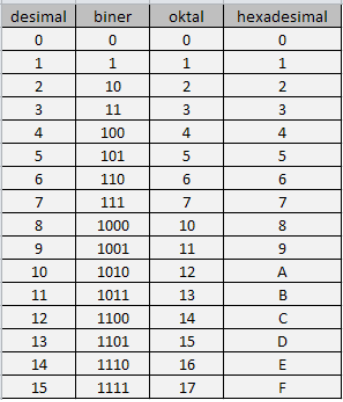
\includegraphics[width=.50\textwidth]{figures/sistem_bilangan.png}
 \caption{Sistem Bilangan}\label{fig:inputchapter}
\end{figure}

\end{enumerate}

\subsection{Tipe Data Floting Point}
Tipe data float (disebut juga tipe data floating point, atau real number) adalah tipe data angka yang memiliki bagian desimal di akhir angka, atau memiliki floating point (floating point adalah istilah dalam bahasa inggris untuk menyebut tanda “titik” yang menandakan bilangan desimal). Contoh angka float adalah seperti: 0,9 atau 3,14. Tipe data float cocok digunakan untuk variabel yang akan berisi angka pecahan, seperti nilai IPK, hasil pembagian, atau hasil komputasi numerik yang angkanya tidak bisa ditampung oleh data integer.
\subsection{Tipe Data String}
Tipe data String adalah tipe data untuk teks yang merupakan gabungan huruf, angka, whitespace (spasi), dan berbagai karakter. Fungsi ini digunakan untuk membuat identifier String/teks. Data string ditulis dengan mengapit data string tersebut dengan tanda petik tunggal atau tanda petik ganda. Tanda petik tunggal umumnya digunakan sebagai konstanta string.
\subsection{Tipe Data Boolean}
Tipe data boolean sebenarnya sangat sederhana. Tipe data ini hanya bisa diisi dengan salah satu dari 2 nilai: TRUE atau FALSE. Tipe data boolean banyak dipakai dalam percabangan kode program, atau untuk memutuskan apa yang harus dijalankan pada sebuah kondisi if else.
\subsection{Tipe Data Objek}
Tipe data dari objek merupakan tipe data baru, merupakan pengembangan PHP untuk mendukung program berorientasi objek. Tipe data objek adalah tipe data yang didalamnya mempunyai data dan method. data yang dipunyai oleh suatu objek populer dengan nama atribut dan method suatu objek umumnya berupa suatu fungsi. 

Data objek didefinisikan dengan membuat definisi kelas terlebih dahulu. Suatu variabel yang bertipe objek diinisialisasi (dideklarasi) dengan menggunakan perintah new kemudian nama objek (berupa nama kelas objek) berikut contohnya:
\lstinputlisting[firstline=1, lastline=17]{src/tipeDataObjek.php}


\section{Operator PHP}
Pada PHP, terdapat banyak operator  beberapa yang sering digunakan.
\subsection{Operator Perbandigan}
Seperti namanya, operator perbandingan digunakan untuk membandingkan beberapa buah nilai pada PHP dan hasilnya berupa booelan true yang berarti benar atau false yang berarti salah.
Contoh:
\begin{lstlisting}
<?php
if ($_POST['password'] == 'admin')
{
	echo 'Login sukses';
}
\end{lstlisting}

\subsection{ Operator PHP Increment dan Decrement}
Operator ini digunakan untuk menambahkan atau mengurangi nilai sebanyak 1 pada suatu variabel. 
\subsection{Perbedaan Pre Increment dan Post Increment}
Pada pre increment, nilai variabel akan ditambahkan 1 baru kemudian siap digunakan, sebaliknya, untuk  post increment, gunakan dulu nilai variabel kemudian baru ditambahkan dengan 1.
Contoh 1:
\begin{lstlisting}
<?php
$nomor = 1;
while($nomor <= 5) {
	echo $nomor++;
}
\end{lstlisting}
Contoh diatas akan menghasilkan angka 12345.

Contoh 2:
\begin{lstlisting}
<?php
$nomor = 1;
while($nomor <= 5) {
	echo ++$nomor;
}
\end{lstlisting}
Contoh diatas akan menghasilkan 23456.
Lihat, perbedaanya terdapat pada ++ sebelum dan sesudah $nomor. 

\subsection{Operator Assignment PHP}
Sesuai namanya Assignment operator ini digunakan untuk memberikan nilai pada suatu variabel. Operator dasarnya adalah tanda sama dengan ( = ). Dalam praktiknya, operator ini sering digunakan ketika menjumlahkan nilai pada suatu perulangan, seperti ketika menjumlahkan data hasil query database.
Contoh:
\begin{lstlisting}
<?php
$sql 	= 'SELECT * FROM sales';
$query 	= mysqli_query($sql);
$total	= 0;
while($row = mysqli_fetch_array($query))
{
	$total += $row['jml_bayar'];
}
\end{lstlisting}

\section{Lingkup Variabel}
Variabel Scope (atau ruang lingkup variabel) adalah jangkauan kode program dimana perintah program masih bisa mengakses sebuah variabel. Variabel menunjukkan keberlakuan dan dikenalinya suatu variabel didalam script. Suatu variabel yang didefinisikan didalam sebuah fungsi maka variabel tersebut hanya akan dikenali dan digunakan hanya dalam fungsi tersebut variabel ini dikenal sebagai variabel lokal. karena hanya dikenal pada fungsi tempat variabel tersebut dinyatakan dan digunakan.

Jika kita mendefenisikan sebuah variabel pada satu file PHP, maka variabel tersebut dapat diakses oleh seluruh kode program pada halaman yang sama. Namun jika variabel tersebut di defenisikan di dalam sebuah fungsi, variabel itu belum tentu bisa diakses dari luar fungsi tersebut. Hal inilah yang dimaksud dengan Variabel Scope. Variabel akan disebut global apabila variabel tersebut dapat dikenali dan digunakan oleh seluruh bagian script tersebut

Variabel yang didefenisikan di dalam sebuah fungsi, secara default tidak dapat diakses oleh kode program di luar fungsi tersebut. Dan begitu juga sebaliknya, variabel yang didefenisikan di luar fungsi, tidak bisa diakses dari dalam fungsi. Berikut jenis variabel berdasarkan lingkupnya:

\subsection{Variabel Global}
\subsection{Variabel Lokal}
\subsection{Variabel Statik}


\chapter{Array}
\section{Array}
Array adalah variabel jamak, yang mempunyai banyak elemen yang diacu dengan satu nama yang sama. Array (atau larik dalam bahasa indonesia) bukanlah tipe data dasar seperti integer atau boolen, Array adalah sebuah tipe data bentukan yang terdiri dari kumpulan tipe data lainnya. Menggunakan array akan memudahkan dalam membuat kelompok data, serta menghemat penulisan dan penggunaan variabel. berikut sebagai contoh
 \begin{lstlisting}
<?php
    $a = array("budi", 20, 58.5);
?>
\end{lstlisting}
Array dalam PHP juga merupakan tipe data, bukan sekedar variabel. Berikut merupakan jenis array dalam PHP:
\subsection{Array Berindeks}
Array berindeks adalah array yang diindeks berdasarkan nomor/angka. Indeks array pada umumnya dimulai dari angka 0. Anda bebas mendefinisikan indeks dengan nilai yang Anda tentukan.

\begin{table}[h]
\caption(Array Berindeks}
\centering
\begin{tabular}
\hline
\textbf{10}&\textbf{20}&\textbf{30}&\textbf{40}&\textbf{50}\\
\hline

\begin{lstlisting}
 $a[0]
\end{lstlisting}  & 

\begin{lstlisting}
 $a[1]
\end{lstlisting} &

\begin{lstlisting}
 $a[2]
\end{lstlisting} &

\begin{lstlisting}
 $a[3]
\end{lstlisting} &

\begin{lstlisting}
 $a[4]
\end{lstlisting}\\
\hline
\end{tabular}
\label{tabel : Array Berindeks}
\end{table}


Contoh diatas menunjukan array dengan 5 buah elemen. Elemen pertama ($a[0]) bernilai 10, elemen
kedua ($a[1]) bernilai 20, dan seterusnya. Dalam array berindeks, antara kunci (indeks) dan nilai tidak
memiliki keterkaitan.

\subsection{Array Asosiatif}
Array asosiatif adalah array yang diindeks berdasarkan nama tertentu. Letak perbedaan antara array berindeks dan array asosiatif adalah hanya terletak pada penamaan indeksnya saja.
\begin{table}[h]
\caption(Array Asosiatif}
\centering
\begin{tabular}{|c|c|c|c|c|}
\hline
\textbf{10}&\textbf{20}&\textbf{30}&\textbf{40}&\textbf{50}\\
\hline

\begin{lstlisting}
 $a["satu"]
\end{lstlisting}  & 

\begin{lstlisting}
 $a["dua"]
\end{lstlisting} &

\begin{lstlisting}
 $a["tiga"]
\end{lstlisting} &

\begin{lstlisting}
 $a["empat"]
\end{lstlisting} &

\begin{lstlisting}
 $a["lima"]
\end{lstlisting}\\
\hline
\end{tabular}
\label{tabel : Array Asosiatif}
\end{table}

Array diindeks berdasarkan nama, bukan berdasarkan nomor. Pada contoh diatas indeks array bertipe string. Pada umumnya array asosiatif digunakan untuk merepresentasikan sesuatu yang kunci dan nilainya memiliki keterkaitan, misalnya sebagai berikut.

\begin{lstlisting}
 <?php
  $kota = array("jkt" => "jakarta", "bdg" => "bandung", "sby" => "surabaya");
 ?>
\end{lstlisting}  


\section{Membuat Array}
Array dapat dibuat melalui dua cara, yaitu dengan menggunakan fungsi array() atau dengan membuat elemen-elemen array dan mengisikan nilai-nilai ke dalam elemen-elemen tersebut secara langsung.
Berikut ini contoh pembuatan array dengan menggunakan fungsi array().

\item{Untuk Array Berindeks}
\begin{lstlisting}
<?php
 $matakuliah = array ("pemograman web", "database", "keamanan jaringan",
 "sistem informasi", "rekayasa perangkat lunak");
 ?>
\end{lstlisting}

\item{Untuk Array Asosiatif}
\begin{lstlisting}
<?php
$detailmk = array ("kode" => "TKB5218", "nama" => "pemograman web 2", "sks" => 2);
?>
\end{lstlisting}

Berikut ini contoh pembuatan array dengan cara langsung membuat variabel array dan mengisikan nilai ke dalamnya.

\item{Untuk array berindeks}
\begin{lstlisting}
<?php 
$matakuliah[0] = "pemograman web"; 
$matakuliah[1] = "database"; 
$matakuliah[2] = "keamanan jaringan"; 
$matakuliah[3] = "sistem informasi"; 
$matakuliah[4] = "rekayasa perangkat lunak"; 
?>
\end{lstlisting}

\item{Untuk array asosiatif}
\begin{lstlisting}
<?php 
$detailmk["kode"] = "TKB5218"; 
$detailmk["nama"] = "pemograman web 2"; 
$detailmk["sks"] = 2; 
?>
\end{lstlisting}

\subsection{File & Direktori}
Dalam management file dan direktori, PHP menyediakan lebih 70 fungsi. Beberapa fungsi utama yang berhubungan dengan management file (create, write, append, dan delete), antara lain : Membuka dan membuat file.
\begin{lstlisting}
fopen ($namafile, $mode);
\end{lstlisting}
Keterangan :
namafile merupakan nama file yang akan dibuat, sedangkan mode merupakan mode akses file. Contoh:
\begin{lstlisting}
<?php
$namafile = "data.txt";
$handle = fopen ($namafile, "mode");
if (!handle) {
	echo "<b>File yang ada buat belum ada</b>";
} else {
	echo "<b>File telah berhasil dibuka</b>";
}
fclose($handle);
?>
\end{lstlisting}


\subsection{Pemrograman Berorientasi Objek Dalam PHP }
PHP pada awalnya hanya sekumpulan script sederhana. Dalam perkembangannya, dapat ditambahkan berbagai fitur pemrograman berorientasi objek. Hal ini dimulai sejak PHP 4. Dengan lahirnya PHP 5, fitur-fitur pemrograman berorientasi objek semakin mantap dan semakin cepat. Dengan PHP 7, script yang menggunakan konsep object-oriented akan lebih cepat dan lebih efisien.
\par
Pemrograman berorientasi objek atau object-oriented programming (OOP) merupakan suatu inovasi dalam pemrograman yang menggunakan object dan class. Saat ini konsep OOP sudah semakin berkembang. Hampir setiap perguruan tinggi di dunia mengajarkan konsep OOP ini pada mahasiswanya. Pemrograman yang banyak dipakai dalam penerapan konsep OOP adalah Java dan C++. OOP bukanlah sekedar cara penulisan sintaks program yang berbeda, namun dapat lebih dari itu, OOP merupakan cara pandang dalam menganalisa sistem dan permasalahan pemrograman. Dalam OOP, setiap bagian dari program adalah object. Sebuah object mewakili suatu bagian program yang akan diselesaikan. Beberapa konsep OOP dasar, antara lain :
\begin{enumerate}
\item Encapsulation (Class dan Object)
\item Inheritance (Penurunan sifat)
\item Polymorphisme
\end{enumerate}
\par
PHP khususnya PHP 7 sudah mendukung beberapa konsep OOP. Akan tetapi PHP 7 tidak mendukung konsep Multiple-inheritance dan polymorphisme.

\subsection{ Object Dan Class}
Bagian dasar dari program yang berorientasi objek adalah objects. Secara tidak langsung  kita dapat memahami mengenai object ini. Sebagai contoh, sebuah mobil adalah objek. Sebuah mobil mempunyai properties atau bagian-bagian di dalamnya, seperti warna, mesin, roda, pintu dsb. Sebuah mobil juga dapat melakukan sesuatu, seperti mengisi bensin, menyalakan mesin, berjalan, mengerem dsb. 
\par
Biasanya object adalah sebuah kata benda. Orang adalah object. Demikian juga mobil, pohon, bunga, komputer, TV, buku dsb. Namun, object tidak selamanya sebuah objek fisik. Bisa saja sebuah benda abstrak, seperti account bank, sebuah file di komputer, database, pesan email, acara TV, dsb. 
Class merupakan penjelasan atau deskripsi dari object. Di dalam class, terdapat penjelasan tentang suatu object termasuk properties yang dimilikinya dan kelakuan atau method yang bisa dilakukan oleh object. Sebagai contoh, class Orang. Class Orang tentu setidaknya memiliki beberapa bagian seperti tangan, kaki, mata, telinga dsb. Class Orang juga setidaknya harus bisa jalan, bisa loncat, bisa lari, bisa melihat, bisa bicara dsb. 
\par
Salah satu keuntungan program didefinisikan dengan konsep OOP adalah adanya pengkapsulan (encapsulation) program dalam class dan object, dimana sang programmer yang menggunakan class tidak perlu mengetahui isi dan jalannya class secara detail, hanya perlu tahu bagaimana cara menggunakannya. Sama halnya dengan sebuah mobil misalnya. Seorang pemilik mobil tentunya tidak perlu mengetahui bagian-bagian mobil secara menyeluruh. Dia tidak perlu mengetahui bagaimana mesin mobil melakukan pembakaran dan bagaimana mesin mobil bisa menggerakkan roda, dsb. Dia hanya perlu tahu bagaimana cara menjalankan mobil, bagaimana menghentikan mobil, dan fungsi mobil lainnya. 


\subsection{Mengakses Elemen Array}
Setelah array dibuat, langkah selanjutnya adalah mengakses nilai-nilai yang terkandung di dalamnya.
Cara mengakses elemen array sangatlah sederhana. Karena elemen array berupa nilai, maka kita dapat
memperlakukannya seperti layaknya variabel.
Kita dapat menempatkan nilai yang diakses ke dalam suatu variabel atau dapat juga diproses secara
langsung baik dalam perhitungan maupun ditampilkan langsung.
Berikut ini adalah contoh mengakses nilai array ke dalam suatu variabel.
\lstinputlisting[firstline=1, lastline=9]{src/array.php}

Berikut ini adalah contoh mengakses elemen array secara langsung
\lstinputlisting[firstline=1, lastline=23]{src/akses_array.php}


\chapter{SQL}
\section{E-Logbook}
E-Logbook adalah sebuah buku elektronik untuk mencatat catatan/dokumen penting secara detail setiap aktivitas yang berisi masalah-masalah yang membutuhkan tindak lanjut dari pihak yang terlibat dalam satu hari penuh. Seluruh pegawai sebaiknya membaca buku ini agar mengetahui kegiatan, kerusakan, dan target pekerjaan apa saja yang dilakukan hari sebelumnya. Ada beberapa manfaat e-logbook antara lain:
\begin{enumerate}
\item bahan bukti untuk merekap seluruh aktivitas
\item bahan pembuatan laporan kegiatan
\item alat untuk memudahkan pegawai dalam merekap kegiatan
 \end{enumerate}

Hal yang perlu di isi dalam e-logbook ini antara lain:
\begin{enumerate}
\item Hari, tanggal dan tahun
\item Nama pegawai yang dinas pada hari tersebut
\item Nama vendor yang dinas pada hari tersebut
\item Penerbangan hari ini
\item Kegiatan
\item Kerusakan
\item Target pekerjaan
\end{enumerate}

\section{Pemrograman Berorientasi Objek Dalam PHP }
PHP pada awalnya hanya sekumpulan script sederhana. Dalam perkembangannya, dapat ditambahkan berbagai fitur pemrograman berorientasi objek. Hal ini dimulai sejak PHP 4. Dengan lahirnya PHP 5, fitur-fitur pemrograman berorientasi objek semakin mantap dan semakin cepat. Dengan PHP 7, script yang menggunakan konsep object-oriented akan lebih cepat dan lebih efisien.
\par
Pemrograman Berorientasi Objek atau Object Oriented Programming (OOP) adalah salah satu cara membuat program dengan memecah menjadi beberapa modul-modul sederhana yang kita sebut sebagai objek. Akan tetapi, setiap memiliki fungsi dan tugas tersendiri. Saat ini OOP telah menjadi sebuah standar dalam dunia pemrograman, termasuk bahasa pemrograman PHP. Kita dapat membuat program PHP walaupun tanpa OOP sama sekali, namun programmer akan beralih menggunakan OOP karena konsepnya yang fleksibel. 
\newline
\textbf{Class}
\newline
Class adalah 'bentuk kasar' dari objek. Class digunakan untuk membuat sebuah kerangka dasar. Yang kita pakai nantinya adalah hasil cetakan dari class yaitu objek. Dalam PHP, penulisan class dapat diawali dengan keyword class kemudian nama dari class tersebut. Aturan penulisan class sama seperti aturan variabel dalam PHP yaitu diawali dengan huruf atau underscore untuk karakter utama, setelahnya dapat berupa selain huruf pada karakter kedua dan selanjutnya.  Isi dari class yang berada di dalam kurung kurawal. Contoh:
\begin{lstlisting}
<?php
class motor {
   // isi dari class test.
}
?>
\end{lstlisting}
\textbf{Property}
\newline
Property atau atribut adalah data yang terdapat di dalam sebuah class. Dalam PHP, aturan tentang tata cara penamaan property ini sama dengan penamaan variabel. Contoh:
\begin{lstlisting}
<?php
class laptop {
   var $pemakai;
   var $merk;
   var $tipe;
   // lanjutan isi dari class motor..
}
?>
\end{lstlisting}
Dari contoh diatas \$pemakai, \$merk, dan \$tipe adalah property dari class motor. Seperti yang kita lihat, penulisan property di dalam PHP sama dengan variabel yaitu dalam penggunaan tanda dollar (\$). Ingat sebuah class tidak harus mempunyai property.

\newline
\textbf{Method}
\newline
Method adalah tindakan apa yang ingin kita lakukan di dalam class. Jika kita menggunakan analogi sebuah motor maka contoh method yaitu: menghidupkan motor, mematikan motor, memvariasi motor, berbagai tindakan lainnya. Method pada dasarnya function atau fungsi yang berada di dalam class. Contoh:
\begin{lstlisting}
<?php
class motor {
   function menghidupkan_motor() {
   //... isi dari method menghidupkan_motor
   }
 
   function memvariasi_motor() {
   //... isi dari method memvariasi_motor
   }
 
   ... //isi dari class motor
}
?>
\end{lstlisting}

Dari contoh di atas, function menghidupkan\_motor() dan function memvariasi\_motor() adalah method dari class motor. Seperti yang kita lihat, bahwa penulisan method di dalam PHP sama dengan cara penulisan function. Sebuah class tidak harus memiliki method.

\newline
\textbf{Object}
\newline
Object atau Objek adalah hasil atau output dari class. Jika kita menggunakan analogi motor, maka objek adalah motor\_honda, motor\_yamaha, motor\_kawasaki, dan lain-lain. Contoh:
\begin{lstlisting}
<?php
class motor {
   //... isi dari class motor
   }
 
$motor_honda = new motor();
$motor_kawasaki = new motor();
?>
\end{lstlisting}
\subsubsection{Cara Mebuat Objek PHP}
\newline
Istilah objek dalam OOP tediri dari class, property, method dan object. Contoh objek dalam PHP:
\begin{lstlisting}
<?php
// membuat class motor
class motor {
  
   // buat property untuk class motor
   var $pemakai;
   var $merk;
   var $tipe;
  
   // buat method untuk class motor
   function menghidupkan_motor() {
     return "Menghidupkan Motor";
   
   function memvariasi_motor() {
     return "Memvariasi Motor";
   }
}
  
// buat objek dari class motor
$motor_honda = new laptop();
?>
\end{lstlisting}

Dari contoh diatas, kita telah membuat class dengan nama motior, selain class kita juga membuat property, method, dan objeknya. 

\subsubsection{Cara Mengakses Objek PHP}
\newline
Cara mengakses objek dalam PHP ini terdiri dari objek, property, dan method. Contoh:
\begin{lstlisting}
<?php
// membuat class motor
class motor {
  
   // membuat property untuk class motor
   var $pemakai;
   var $merk;
   var $tipe;
  
   // membuat method untuk class motor
   function menghidupkan_motor() {
     return "Menghidupkan Motor";
    }
   function memvariasi_motor() {
     return "Memvariasi Motor";
   }
}
  
// membuat objek dari class motor
$motor_honda = new motor();
  
// atur property
$motor_honda>pemakai="Luqman";
$motor_honda->merk="Beat";
$motor_honda->tipe="CBS";
  
// tampilkan property
echo $motor_honda->pemakai;
echo "<br />";
echo $motor_honda->merk;
echo "<br />";
echo $motor_honda->tipe;
echo "<br />";
  
// tampilkan method
echo $motor_honda->menghidupkan_motor();
echo "<br />";
echo $memvariasi_motor->memvariasi_motor();
?>
\end{lstlisting}

Hasil dari contoh diatas adalah sebagai berikut:
\begin{lstlisting}
Luqman
Beat
CBS
Menghidupkan Motor
Memvariasi Motor
\end{lstlisting}


\subsection{Database}
Basis Data (database) adalah sebuah kumpulan data yang dapat disimpan secara terstruktur di dalam komputer untuk diolah atau di manupulasi menggunakan sebuah program aplikasi agar dapat menghasilkan informasi. Basis data ini merupakan bagian yang sangat penting dalam pembuatan sistem informasi karena berfungsi sebagai pusat penyimpanan data yang akan di organisasikan. Proses memasukan dan mengolah data dari media penyimpanan membutuhkan media perangkat lunak yang disebut DBMS (Database Management System). DBMS adalah sistem perangkat lunak yan dapat mengorganisasikan data secara praktis dan efisien.
\par
Beberapa perangkat lunak atau DBMS yang sering digunakan dalam pembuatan aplikasi antara lain:
\begin{enumerate}
\item MySQL - https://www.mysql.com/
\item Oracle - https://www.oracle.com/id/index.html
\item Microsoft SQL Server - https://www.microsoft.com/en-us/sql-server/sql-server-downloads
\item MariaDB - https://mariadb.org/
\end{enumerate}
Akan tetapi, dalam pembuatan aplikasi disini kita menggunakan MySQL.
\newline
MySQL adalah sistem manajemen basis data relasional open-source (RDBMS). Namanya adalah kombinasi dari "My", nama co-founder putri Michael Widenius, dan "SQL", singkatan dari Structured Query Language. MySQL adalah perangkat lunak bebas dan sumber terbuka di bawah ketentuan GNU General Public License, dan juga tersedia di bawah berbagai lisensi kepemilikan. MySQL dimiliki dan disponsori oleh perusahaan Swedia MySQL AB, yang dibeli oleh Sun Microsystems (sekarang Oracle Corporation). Pada 2010, ketika Oracle mengakuisisi Sun, Widenius melakukan forked pada proyek open-source MySQL untuk membuat MariaDB. MySQL adalah komponen dari tumpukan perangkat lunak aplikasi web LAMP (dan lainnya), yang merupakan akronim untuk Linux, Apache, MySQL, Perl / PHP / Python. MySQL digunakan oleh banyak aplikasi web berbasis database, termasuk Drupal, Joomla, phpBB, dan WordPress. MySQL juga digunakan oleh banyak situs web populer, termasuk Facebook, Twitter, Flickr, dan YouTube. 
\par
Untuk PHP kita menggunakan phpMyAdmin. phpMyAdmin adalah alat perangkat lunak gratis yang ditulis dalam PHP, dimaksudkan untuk menangani administrasi MySQL melalui Web. phpMyAdmin mendukung berbagai operasi di MySQL dan MariaDB. Operasi yang sering digunakan (mengelola basis data, tabel, kolom, hubungan, indeks, pengguna, izin, dll) dapat dilakukan melalui antarmuka pengguna, sementara Anda masih memiliki kemampuan untuk secara langsung menjalankan pernyataan SQL apa pun.

\subsection{Mengaktifkan MySQLi}
Kenapa disini kita membahas tentang cara mengaktifkan MySQLi karena PHP 5 keatas default-nya menggunakan platform MySQLi untuk menggunakan berbagai fungsi pada database MySQL. MySQLi adalah sebuah class di PHP, jadi pastikan bahwa versi PHP kita sudah 5 keatas yaa.
Keunggulan menggunakan MySQLi ketimbang dengan MySQL:
\begin{enumerate}
\item Dukungan baru untuk keperluan transaksi
\item Prosedur interface
\item Susunan laporan lebih tersusun
\item Debugging lebih ditingkatkan
\item Dapat memproses dalam waktu yang lebih singkat
\end{enumerate}

Nah itu beberapa keunggulan menggunakan MySQLi. Dan sekarang kita akan membahas cara mengaktifkan MySQLi pada PHP.
Untuk mengaktifkan MySQLi, langkah pertama update dahulu versi PHP kita ke PHP 5 keatas. kemudian cari file php.ini biasanya terdapat di folder C lalu folder xampp lalu folder php kemudian buka file php.ini menggunakan editor seperti notepad++, sublime text, dan adobe dreamweaver. Tambahkan skrip extension=php\_mysqli.dll pada file php.ini. Namun pada file php.ini sudah ada skrip extension=php\_mysqli.dll dan terdapat tanda ; (tanpa tanda kutip) di depanya, maka kita cukup menghapus tanda ; tersebut lalu simpan file php.ini yang sudah di edit. Jangan lupa untuk restart server apachenya.


\subsection{Membuat Database}
Secara umum, tipe website bisa dibedakan menjadi dua yaitu web statis dan web dinamis. Web statis adalah web yang tetap dalam arti tampilan, navigasi, dan konten tidak dapat berubah dengan otomatis. Ketika kita ingin mengupdate sebuah kegiatan akan tetapi kita harus membuka file yang aslinya. Umumnya kegiatan yang ditampillkan tetap untuk jangka waktu satu hari - satu hari. Tipe website ini biasanya hanya berupa tag html saja, jadi diperlukan database yang digunakan untuk menyimpan data.
\par
Selain memanfaatkan tag html, website yang menggunakan flash juga bisa dikategorikan sebagai web statis, meskipun ada sebagian kecil yang sudah memiliki database dalam mengelola konten tidak perlu membuka sebuah file tertentu namum hanya menambahkan pada form yang telah disiapkan dan tersimpan di database. Sama halnya dengan e-logbook ini harus ada database yang dibuat.
\begin{enumerate}
\item Untuk membuat database kita pertama kali harus membuka aplikasi XAMPP yang sudah terinstall dan klik start pada Apache serta MySQL.

 \begin{figure}[h]
\centering
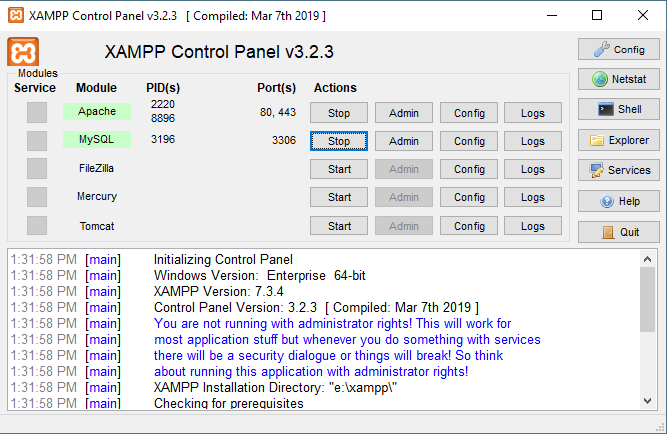
\includegraphics[scale=0.5]{figures/controlpanel}
\caption{XAMPP Control Panel}
\end{figure}

\item Jika sudah berjalan maka selanjutnya buka web browser kesayangan kita lalu ketikan https://localhost/phpmyadmin

 \begin{figure}[h]
\centering
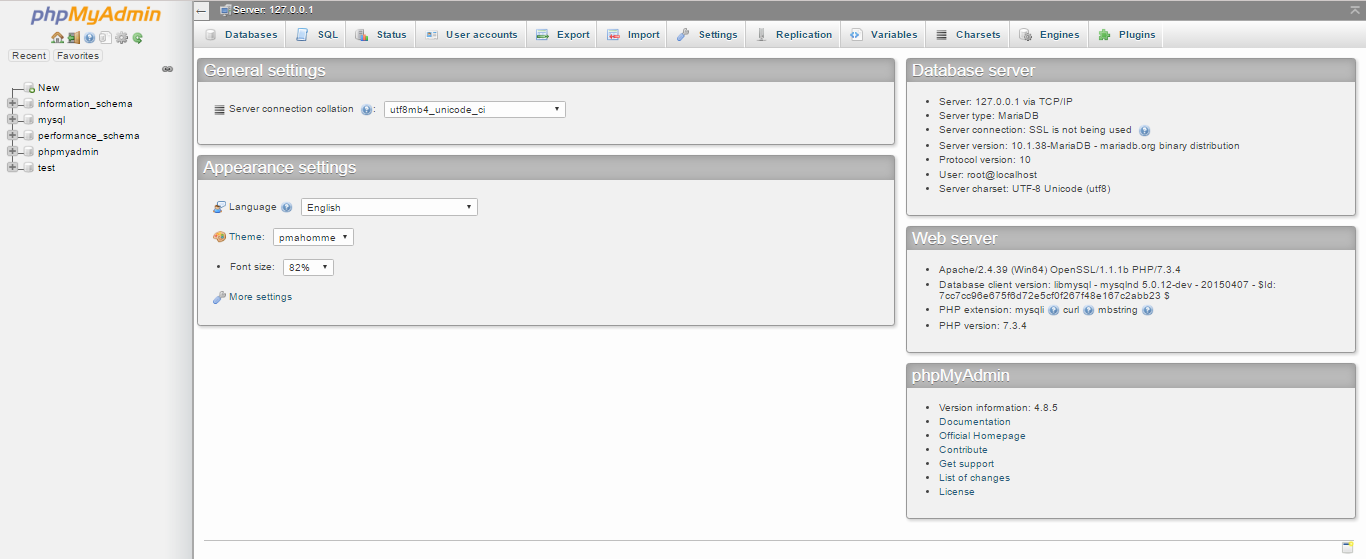
\includegraphics[scale=0.35]{figures/phpmyadmin}
\caption{Halaman Utama}
\end{figure}

\item Setelah itu, klik databases lalu ketikkan elban lalu klik create

 \begin{figure}[h]
\centering
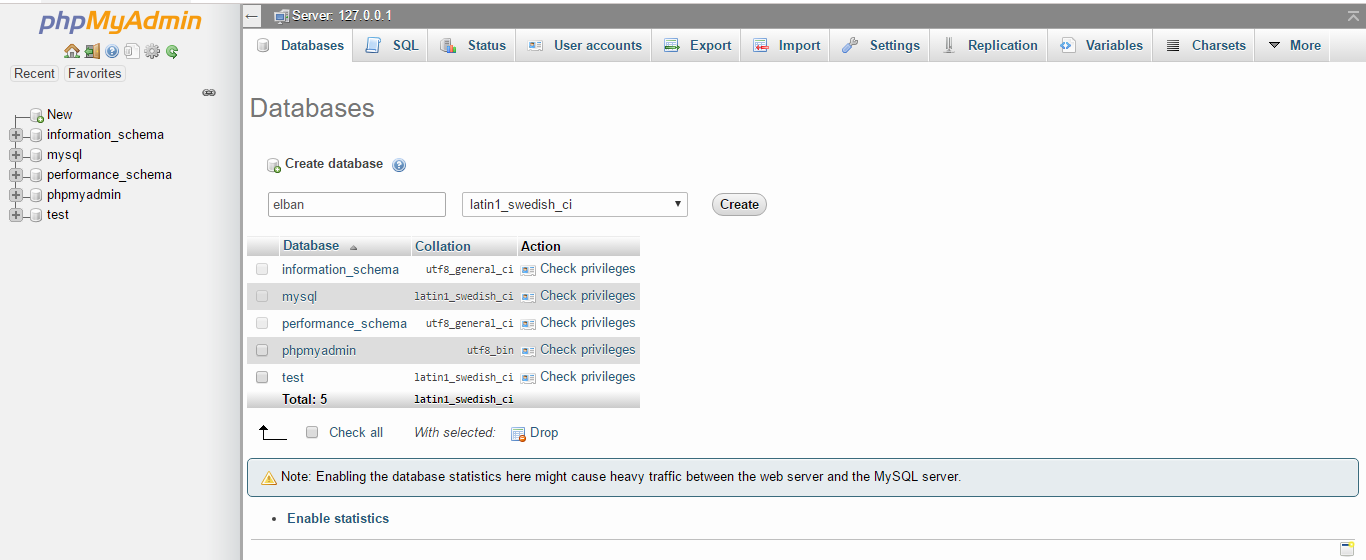
\includegraphics[scale=0.35]{figures/databases}
\caption{Create Database}
\end{figure}

\item Setelah database dibuat lalu belum ada table, klik SQL lalu masukan codingan berikut

\begin{lstlisting}
CREATE TABLE IF NOT EXISTS `logbook` (
  `id_logbook` int(10) NOT NULL,
  `tanggal` date NOT NULL,
  `petugas` varchar(100) NOT NULL,
  `vendor` varchar(100) NOT NULL,
  `penerbangan` varchar(100) NOT NULL,
  `kegiatan` varchar(500) NOT NULL,
  `point_kerusakan` varchar(200) NOT NULL,
  `target_pekerjaan` varchar(200) NOT NULL,
  `id_user` tinyint(1) NOT NULL
) ENGINE=InnoDB AUTO_INCREMENT=4 DEFAULT CHARSET=latin1;

--
-- Dumping data for table `logbook`
--

INSERT INTO `logbook` (`id_logbook`, `tanggal`, `petugas`, `vendor`, `penerbangan`, `kegiatan`, `point_kerusakan`, `target_pekerjaan`, `id_user`) VALUES
(2, '2019-03-31', 'M. Arif S, Vania & Rismayadi', 'Anto (CUPPS) Hisyam', 'Citylink KJT - KNO', 'PM di SCP 2 Inter Line 1', 'Master Clok Gate 4, XRAY BHS Internasional', 'Master Clock Gate 4', 12),
(3, '2019-03-28', 'M. Arif S & Vania', 'Anto (CUPPS) Hisyam', 'KJT - KNO (Cancelled)', 'PM', 'Master clock gate 4 off', 'Master CloCk gate 4', 12);

-- --------------------------------------------------------

--
-- Table structure for table `pegawai`
--

CREATE TABLE IF NOT EXISTS `pegawai` (
  `id_pegawai` int(10) NOT NULL,
  `pegawai` varchar(100) NOT NULL
) ENGINE=InnoDB AUTO_INCREMENT=16 DEFAULT CHARSET=latin1;

--
-- Dumping data for table `pegawai`
--

INSERT INTO `pegawai` (`id_pegawai`, `pegawai`) VALUES
(1, 'M. Arif S'),
(2, 'M. Arif S & Vania'),
(3, 'M. Arif S, Vania & Hafiz'),
(4, 'M. Arif S, Vania & Rismayadi'),
(5, 'M. Arif S & Hafiz'),
(6, 'M. Arif S & Rismayadi'),
(7, 'M. Arif S, Vania, Hafiz & Rismayadi'),
(8, 'Vania'),
(9, 'Vania & Hafiz'),
(10, 'Vania & Rismayadi'),
(11, 'Vania, Hafiz & Rismayadi'),
(12, 'Hafiz'),
(13, 'Hafiz & Rismayadi'),
(14, 'Rismayadi'),
(15, 'M. Arif S, Hafiz & Rismayadi');

-- --------------------------------------------------------

--
-- Table structure for table `user`
--

CREATE TABLE IF NOT EXISTS `user` (
  `id_user` tinyint(2) NOT NULL,
  `username` varchar(30) NOT NULL,
  `password` varchar(35) NOT NULL,
  `nama` varchar(50) NOT NULL,
  `alamat` varchar(150) NOT NULL,
  `hp` varchar(20) NOT NULL,
  `level` tinyint(1) NOT NULL
) ENGINE=InnoDB AUTO_INCREMENT=14 DEFAULT CHARSET=latin1;

--
-- Dumping data for table `user`
--

INSERT INTO `user` (`id_user`, `username`, `password`, `nama`, `alamat`, `hp`, `level`) VALUES
(1, 'admin', '21232f297a57a5a743894a0e4a801fc3', 'Luqman Nurfajri', 'Ciwarugotham', '089634530333', 1),
(13, 'vania', '081c2ce8528c443cc4be69d4096c9778', 'Vania R', 'Kertajati', '-', 1);

--
-- Indexes for dumped tables
--

--
-- Indexes for table `logbook`
--
ALTER TABLE `logbook`
  ADD PRIMARY KEY (`id_logbook`);

--
-- Indexes for table `pegawai`
--
ALTER TABLE `pegawai`
  ADD PRIMARY KEY (`id_pegawai`);

--
-- Indexes for table `user`
--
ALTER TABLE `user`
  ADD PRIMARY KEY (`id_user`);

--
-- AUTO_INCREMENT for dumped tables
--

--
-- AUTO_INCREMENT for table `logbook`
--
ALTER TABLE `logbook`
  MODIFY `id_logbook` int(10) NOT NULL AUTO_INCREMENT,AUTO_INCREMENT=4;
--
-- AUTO_INCREMENT for table `pegawai`
--
ALTER TABLE `pegawai`
  MODIFY `id_pegawai` int(10) NOT NULL AUTO_INCREMENT,AUTO_INCREMENT=16;
--
-- AUTO_INCREMENT for table `user`
--
ALTER TABLE `user`
  MODIFY `id_user` tinyint(2) NOT NULL AUTO_INCREMENT,AUTO_INCREMENT=14;
\end{lstlisting}

\end{enumerate}

\chapter{Object Oriented Programming}
\section{E-Logbook}
E-Logbook adalah sebuah buku elektronik untuk mencatat catatan/dokumen penting secara detail setiap aktivitas yang berisi masalah-masalah yang membutuhkan tindak lanjut dari pihak yang terlibat dalam satu hari penuh. Seluruh pegawai sebaiknya membaca buku ini agar mengetahui kegiatan, kerusakan, dan target pekerjaan apa saja yang dilakukan hari sebelumnya. Ada beberapa manfaat e-logbook antara lain:
\begin{enumerate}
\item bahan bukti untuk merekap seluruh aktivitas
\item bahan pembuatan laporan kegiatan
\item alat untuk memudahkan pegawai dalam merekap kegiatan
 \end{enumerate}

Hal yang perlu di isi dalam e-logbook ini antara lain:
\begin{enumerate}
\item Hari, tanggal dan tahun
\item Nama pegawai yang dinas pada hari tersebut
\item Nama vendor yang dinas pada hari tersebut
\item Penerbangan hari ini
\item Kegiatan
\item Kerusakan
\item Target pekerjaan
\end{enumerate}

\section{Pemrograman Berorientasi Objek Dalam PHP }
PHP pada awalnya hanya sekumpulan script sederhana. Dalam perkembangannya, dapat ditambahkan berbagai fitur pemrograman berorientasi objek. Hal ini dimulai sejak PHP 4. Dengan lahirnya PHP 5, fitur-fitur pemrograman berorientasi objek semakin mantap dan semakin cepat. Dengan PHP 7, script yang menggunakan konsep object-oriented akan lebih cepat dan lebih efisien.
\par
Pemrograman Berorientasi Objek atau Object Oriented Programming (OOP) adalah salah satu cara membuat program dengan memecah menjadi beberapa modul-modul sederhana yang kita sebut sebagai objek. Akan tetapi, setiap memiliki fungsi dan tugas tersendiri. Saat ini OOP telah menjadi sebuah standar dalam dunia pemrograman, termasuk bahasa pemrograman PHP. Kita dapat membuat program PHP walaupun tanpa OOP sama sekali, namun programmer akan beralih menggunakan OOP karena konsepnya yang fleksibel. 
\newline
\textbf{Class}
\newline
Class adalah 'bentuk kasar' dari objek. Class digunakan untuk membuat sebuah kerangka dasar. Yang kita pakai nantinya adalah hasil cetakan dari class yaitu objek. Dalam PHP, penulisan class dapat diawali dengan keyword class kemudian nama dari class tersebut. Aturan penulisan class sama seperti aturan variabel dalam PHP yaitu diawali dengan huruf atau underscore untuk karakter utama, setelahnya dapat berupa selain huruf pada karakter kedua dan selanjutnya.  Isi dari class yang berada di dalam kurung kurawal. Contoh:
\begin{lstlisting}
<?php
class motor {
   // isi dari class test.
}
?>
\end{lstlisting}
\textbf{Property}
\newline
Property atau atribut adalah data yang terdapat di dalam sebuah class. Dalam PHP, aturan tentang tata cara penamaan property ini sama dengan penamaan variabel. Contoh:
\begin{lstlisting}
<?php
class laptop {
   var $pemakai;
   var $merk;
   var $tipe;
   // lanjutan isi dari class motor..
}
?>
\end{lstlisting}
Dari contoh diatas \$pemakai, \$merk, dan \$tipe adalah property dari class motor. Seperti yang kita lihat, penulisan property di dalam PHP sama dengan variabel yaitu dalam penggunaan tanda dollar (\$). Ingat sebuah class tidak harus mempunyai property.

\newline
\textbf{Method}
\newline
Method adalah tindakan apa yang ingin kita lakukan di dalam class. Jika kita menggunakan analogi sebuah motor maka contoh method yaitu: menghidupkan motor, mematikan motor, memvariasi motor, berbagai tindakan lainnya. Method pada dasarnya function atau fungsi yang berada di dalam class. Contoh:
\begin{lstlisting}
<?php
class motor {
   function menghidupkan_motor() {
   //... isi dari method menghidupkan_motor
   }
 
   function memvariasi_motor() {
   //... isi dari method memvariasi_motor
   }
 
   ... //isi dari class motor
}
?>
\end{lstlisting}

Dari contoh di atas, function menghidupkan\_motor() dan function memvariasi\_motor() adalah method dari class motor. Seperti yang kita lihat, bahwa penulisan method di dalam PHP sama dengan cara penulisan function. Sebuah class tidak harus memiliki method.

\newline
\textbf{Object}
\newline
Object atau Objek adalah hasil atau output dari class. Jika kita menggunakan analogi motor, maka objek adalah motor\_honda, motor\_yamaha, motor\_kawasaki, dan lain-lain. Contoh:
\begin{lstlisting}
<?php
class motor {
   //... isi dari class motor
   }
 
$motor_honda = new motor();
$motor_kawasaki = new motor();
?>
\end{lstlisting}
\subsubsection{Cara Mebuat Objek PHP}
\newline
Istilah objek dalam OOP tediri dari class, property, method dan object. Contoh objek dalam PHP:
\begin{lstlisting}
<?php
// membuat class motor
class motor {
  
   // buat property untuk class motor
   var $pemakai;
   var $merk;
   var $tipe;
  
   // buat method untuk class motor
   function menghidupkan_motor() {
     return "Menghidupkan Motor";
   
   function memvariasi_motor() {
     return "Memvariasi Motor";
   }
}
  
// buat objek dari class motor
$motor_honda = new laptop();
?>
\end{lstlisting}

Dari contoh diatas, kita telah membuat class dengan nama motior, selain class kita juga membuat property, method, dan objeknya. 

\subsubsection{Cara Mengakses Objek PHP}
\newline
Cara mengakses objek dalam PHP ini terdiri dari objek, property, dan method. Contoh:
\begin{lstlisting}
<?php
// membuat class motor
class motor {
  
   // membuat property untuk class motor
   var $pemakai;
   var $merk;
   var $tipe;
  
   // membuat method untuk class motor
   function menghidupkan_motor() {
     return "Menghidupkan Motor";
    }
   function memvariasi_motor() {
     return "Memvariasi Motor";
   }
}
  
// membuat objek dari class motor
$motor_honda = new motor();
  
// atur property
$motor_honda>pemakai="Luqman";
$motor_honda->merk="Beat";
$motor_honda->tipe="CBS";
  
// tampilkan property
echo $motor_honda->pemakai;
echo "<br />";
echo $motor_honda->merk;
echo "<br />";
echo $motor_honda->tipe;
echo "<br />";
  
// tampilkan method
echo $motor_honda->menghidupkan_motor();
echo "<br />";
echo $memvariasi_motor->memvariasi_motor();
?>
\end{lstlisting}

Hasil dari contoh diatas adalah sebagai berikut:
\begin{lstlisting}
Luqman
Beat
CBS
Menghidupkan Motor
Memvariasi Motor
\end{lstlisting}


\subsection{Database}
Basis Data (database) adalah sebuah kumpulan data yang dapat disimpan secara terstruktur di dalam komputer untuk diolah atau di manupulasi menggunakan sebuah program aplikasi agar dapat menghasilkan informasi. Basis data ini merupakan bagian yang sangat penting dalam pembuatan sistem informasi karena berfungsi sebagai pusat penyimpanan data yang akan di organisasikan. Proses memasukan dan mengolah data dari media penyimpanan membutuhkan media perangkat lunak yang disebut DBMS (Database Management System). DBMS adalah sistem perangkat lunak yan dapat mengorganisasikan data secara praktis dan efisien.
\par
Beberapa perangkat lunak atau DBMS yang sering digunakan dalam pembuatan aplikasi antara lain:
\begin{enumerate}
\item MySQL - https://www.mysql.com/
\item Oracle - https://www.oracle.com/id/index.html
\item Microsoft SQL Server - https://www.microsoft.com/en-us/sql-server/sql-server-downloads
\item MariaDB - https://mariadb.org/
\end{enumerate}
Akan tetapi, dalam pembuatan aplikasi disini kita menggunakan MySQL.
\newline
MySQL adalah sistem manajemen basis data relasional open-source (RDBMS). Namanya adalah kombinasi dari "My", nama co-founder putri Michael Widenius, dan "SQL", singkatan dari Structured Query Language. MySQL adalah perangkat lunak bebas dan sumber terbuka di bawah ketentuan GNU General Public License, dan juga tersedia di bawah berbagai lisensi kepemilikan. MySQL dimiliki dan disponsori oleh perusahaan Swedia MySQL AB, yang dibeli oleh Sun Microsystems (sekarang Oracle Corporation). Pada 2010, ketika Oracle mengakuisisi Sun, Widenius melakukan forked pada proyek open-source MySQL untuk membuat MariaDB. MySQL adalah komponen dari tumpukan perangkat lunak aplikasi web LAMP (dan lainnya), yang merupakan akronim untuk Linux, Apache, MySQL, Perl / PHP / Python. MySQL digunakan oleh banyak aplikasi web berbasis database, termasuk Drupal, Joomla, phpBB, dan WordPress. MySQL juga digunakan oleh banyak situs web populer, termasuk Facebook, Twitter, Flickr, dan YouTube. 
\par
Untuk PHP kita menggunakan phpMyAdmin. phpMyAdmin adalah alat perangkat lunak gratis yang ditulis dalam PHP, dimaksudkan untuk menangani administrasi MySQL melalui Web. phpMyAdmin mendukung berbagai operasi di MySQL dan MariaDB. Operasi yang sering digunakan (mengelola basis data, tabel, kolom, hubungan, indeks, pengguna, izin, dll) dapat dilakukan melalui antarmuka pengguna, sementara Anda masih memiliki kemampuan untuk secara langsung menjalankan pernyataan SQL apa pun.

\subsection{Mengaktifkan MySQLi}
Kenapa disini kita membahas tentang cara mengaktifkan MySQLi karena PHP 5 keatas default-nya menggunakan platform MySQLi untuk menggunakan berbagai fungsi pada database MySQL. MySQLi adalah sebuah class di PHP, jadi pastikan bahwa versi PHP kita sudah 5 keatas yaa.
Keunggulan menggunakan MySQLi ketimbang dengan MySQL:
\begin{enumerate}
\item Dukungan baru untuk keperluan transaksi
\item Prosedur interface
\item Susunan laporan lebih tersusun
\item Debugging lebih ditingkatkan
\item Dapat memproses dalam waktu yang lebih singkat
\end{enumerate}

Nah itu beberapa keunggulan menggunakan MySQLi. Dan sekarang kita akan membahas cara mengaktifkan MySQLi pada PHP.
Untuk mengaktifkan MySQLi, langkah pertama update dahulu versi PHP kita ke PHP 5 keatas. kemudian cari file php.ini biasanya terdapat di folder C lalu folder xampp lalu folder php kemudian buka file php.ini menggunakan editor seperti notepad++, sublime text, dan adobe dreamweaver. Tambahkan skrip extension=php\_mysqli.dll pada file php.ini. Namun pada file php.ini sudah ada skrip extension=php\_mysqli.dll dan terdapat tanda ; (tanpa tanda kutip) di depanya, maka kita cukup menghapus tanda ; tersebut lalu simpan file php.ini yang sudah di edit. Jangan lupa untuk restart server apachenya.


\subsection{Membuat Database}
Secara umum, tipe website bisa dibedakan menjadi dua yaitu web statis dan web dinamis. Web statis adalah web yang tetap dalam arti tampilan, navigasi, dan konten tidak dapat berubah dengan otomatis. Ketika kita ingin mengupdate sebuah kegiatan akan tetapi kita harus membuka file yang aslinya. Umumnya kegiatan yang ditampillkan tetap untuk jangka waktu satu hari - satu hari. Tipe website ini biasanya hanya berupa tag html saja, jadi diperlukan database yang digunakan untuk menyimpan data.
\par
Selain memanfaatkan tag html, website yang menggunakan flash juga bisa dikategorikan sebagai web statis, meskipun ada sebagian kecil yang sudah memiliki database dalam mengelola konten tidak perlu membuka sebuah file tertentu namum hanya menambahkan pada form yang telah disiapkan dan tersimpan di database. Sama halnya dengan e-logbook ini harus ada database yang dibuat.
\begin{enumerate}
\item Untuk membuat database kita pertama kali harus membuka aplikasi XAMPP yang sudah terinstall dan klik start pada Apache serta MySQL.

 \begin{figure}[h]
\centering
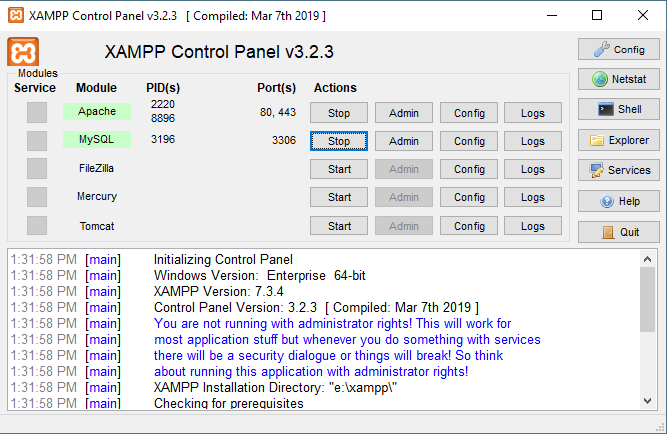
\includegraphics[scale=0.5]{figures/controlpanel}
\caption{XAMPP Control Panel}
\end{figure}

\item Jika sudah berjalan maka selanjutnya buka web browser kesayangan kita lalu ketikan https://localhost/phpmyadmin

 \begin{figure}[h]
\centering
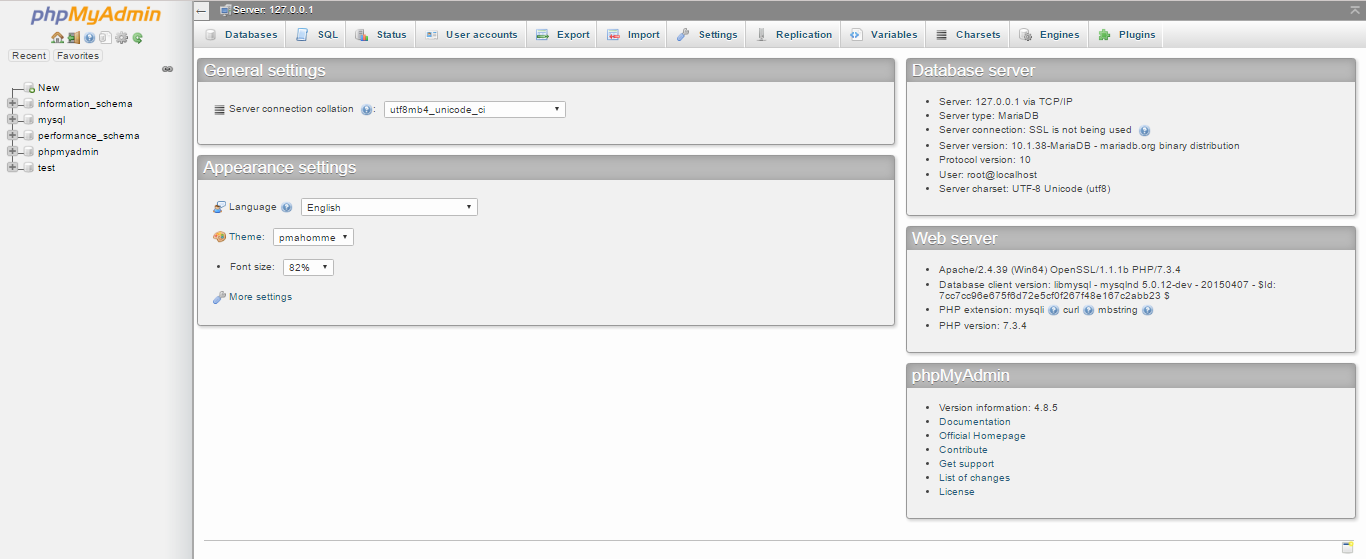
\includegraphics[scale=0.35]{figures/phpmyadmin}
\caption{Halaman Utama}
\end{figure}

\item Setelah itu, klik databases lalu ketikkan elban lalu klik create

 \begin{figure}[h]
\centering
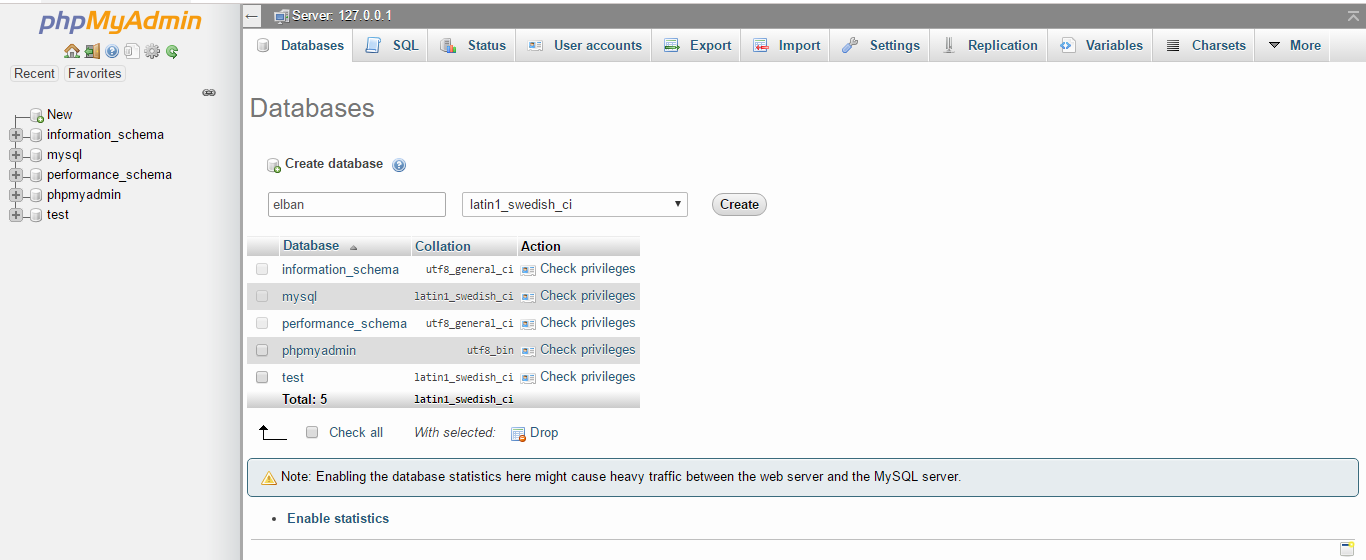
\includegraphics[scale=0.35]{figures/databases}
\caption{Create Database}
\end{figure}

\item Setelah database dibuat lalu belum ada table, klik SQL lalu masukan codingan berikut

\begin{lstlisting}
CREATE TABLE IF NOT EXISTS `logbook` (
  `id_logbook` int(10) NOT NULL,
  `tanggal` date NOT NULL,
  `petugas` varchar(100) NOT NULL,
  `vendor` varchar(100) NOT NULL,
  `penerbangan` varchar(100) NOT NULL,
  `kegiatan` varchar(500) NOT NULL,
  `point_kerusakan` varchar(200) NOT NULL,
  `target_pekerjaan` varchar(200) NOT NULL,
  `id_user` tinyint(1) NOT NULL
) ENGINE=InnoDB AUTO_INCREMENT=4 DEFAULT CHARSET=latin1;

--
-- Dumping data for table `logbook`
--

INSERT INTO `logbook` (`id_logbook`, `tanggal`, `petugas`, `vendor`, `penerbangan`, `kegiatan`, `point_kerusakan`, `target_pekerjaan`, `id_user`) VALUES
(2, '2019-03-31', 'M. Arif S, Vania & Rismayadi', 'Anto (CUPPS) Hisyam', 'Citylink KJT - KNO', 'PM di SCP 2 Inter Line 1', 'Master Clok Gate 4, XRAY BHS Internasional', 'Master Clock Gate 4', 12),
(3, '2019-03-28', 'M. Arif S & Vania', 'Anto (CUPPS) Hisyam', 'KJT - KNO (Cancelled)', 'PM', 'Master clock gate 4 off', 'Master CloCk gate 4', 12);

-- --------------------------------------------------------

--
-- Table structure for table `pegawai`
--

CREATE TABLE IF NOT EXISTS `pegawai` (
  `id_pegawai` int(10) NOT NULL,
  `pegawai` varchar(100) NOT NULL
) ENGINE=InnoDB AUTO_INCREMENT=16 DEFAULT CHARSET=latin1;

--
-- Dumping data for table `pegawai`
--

INSERT INTO `pegawai` (`id_pegawai`, `pegawai`) VALUES
(1, 'M. Arif S'),
(2, 'M. Arif S & Vania'),
(3, 'M. Arif S, Vania & Hafiz'),
(4, 'M. Arif S, Vania & Rismayadi'),
(5, 'M. Arif S & Hafiz'),
(6, 'M. Arif S & Rismayadi'),
(7, 'M. Arif S, Vania, Hafiz & Rismayadi'),
(8, 'Vania'),
(9, 'Vania & Hafiz'),
(10, 'Vania & Rismayadi'),
(11, 'Vania, Hafiz & Rismayadi'),
(12, 'Hafiz'),
(13, 'Hafiz & Rismayadi'),
(14, 'Rismayadi'),
(15, 'M. Arif S, Hafiz & Rismayadi');

-- --------------------------------------------------------

--
-- Table structure for table `user`
--

CREATE TABLE IF NOT EXISTS `user` (
  `id_user` tinyint(2) NOT NULL,
  `username` varchar(30) NOT NULL,
  `password` varchar(35) NOT NULL,
  `nama` varchar(50) NOT NULL,
  `alamat` varchar(150) NOT NULL,
  `hp` varchar(20) NOT NULL,
  `level` tinyint(1) NOT NULL
) ENGINE=InnoDB AUTO_INCREMENT=14 DEFAULT CHARSET=latin1;

--
-- Dumping data for table `user`
--

INSERT INTO `user` (`id_user`, `username`, `password`, `nama`, `alamat`, `hp`, `level`) VALUES
(1, 'admin', '21232f297a57a5a743894a0e4a801fc3', 'Luqman Nurfajri', 'Ciwarugotham', '089634530333', 1),
(13, 'vania', '081c2ce8528c443cc4be69d4096c9778', 'Vania R', 'Kertajati', '-', 1);

--
-- Indexes for dumped tables
--

--
-- Indexes for table `logbook`
--
ALTER TABLE `logbook`
  ADD PRIMARY KEY (`id_logbook`);

--
-- Indexes for table `pegawai`
--
ALTER TABLE `pegawai`
  ADD PRIMARY KEY (`id_pegawai`);

--
-- Indexes for table `user`
--
ALTER TABLE `user`
  ADD PRIMARY KEY (`id_user`);

--
-- AUTO_INCREMENT for dumped tables
--

--
-- AUTO_INCREMENT for table `logbook`
--
ALTER TABLE `logbook`
  MODIFY `id_logbook` int(10) NOT NULL AUTO_INCREMENT,AUTO_INCREMENT=4;
--
-- AUTO_INCREMENT for table `pegawai`
--
ALTER TABLE `pegawai`
  MODIFY `id_pegawai` int(10) NOT NULL AUTO_INCREMENT,AUTO_INCREMENT=16;
--
-- AUTO_INCREMENT for table `user`
--
ALTER TABLE `user`
  MODIFY `id_user` tinyint(2) NOT NULL AUTO_INCREMENT,AUTO_INCREMENT=14;
\end{lstlisting}

\end{enumerate}



\bibliographystyle{IEEEtran} 
%\def\bibfont{\normalsize}
\bibliography{references}


%%%%%%%%%%%%%%%
%%  The default LaTeX Index
%%  Don't need to add any commands before \begin{document}
\printindex


%%%% Making an index
%% 
%% 1. Make index entries, don't leave any spaces so that they
%% will be sorted correctly.
%% 
%% \index{term}
%% \index{term!subterm}
%% \index{term!subterm!subsubterm}
%% 
%% 2. Run LaTeX several times to produce <filename>.idx
%% 
%% 3. On command line, type  makeindx <filename> which
%% will produce <filename>.ind 
%% 
%% 4. Type \printindex to make the index appear in your book.
%% 
%% 5. If you would like to edit <filename>.ind 
%% you may do so. See docs.pdf for more information.
%% 
%%%%%%%%%%%%%%%%%%%%%%%%%%%%%%

%%%%%%%%%%%%%% Making Multiple Indices %%%%%%%%%%%%%%%%
%% 1. 
%% \usepackage{multind}
%% \makeindex{book}
%% \makeindex{authors}
%% \begin{document}
%% 
%% 2.
%% % add index terms to your book, ie,
%% \index{book}{A term to go to the topic index}
%% \index{authors}{Put this author in the author index}
%% 
%% \index{book}{Cows}
%% \index{book}{Cows!Jersey}
%% \index{book}{Cows!Jersey!Brown}
%% 
%% \index{author}{Douglas Adams}
%% \index{author}{Boethius}
%% \index{author}{Mark Twain}
%% 
%% 3. On command line type 
%% makeindex topic 
%% makeindex authors
%% 
%% 4.
%% this is a Wiley command to make the indices print:
%% \multiprintindex{book}{Topic index}
%% \multiprintindex{authors}{Author index}

\end{document}

